\chapter{Diseño e implementación} % Main chapter title

En este capitulo se explican las consideraciones de diseño realizadas junto con detalles de implementación del software que usa el dispositivo.
\label{Chapter3} 

%----------------------------------------------------------------------------------------
%	SECTION 1
%----------------------------------------------------------------------------------------
\section{Desarrollo de \textit{hardware}}
 
\subsection{Estructura Planteada }

Inicialmente basándose en la figura \ref{fig:esquema1} del planeamiento  se pensó en el diseño de una placa con dos sectores aislados, el sector del microcontrolador por un lado y el sector de medición en otro sector.

En el sector del microcontrolador se encontrarían, ademas del micro principal, los integrados de comunicación y las salidas.

Por otro lado el sector de medición debía manejar alta tensión, por lo que en este sector es donde irían los arreglos analógicos para lograr la medición. 

También se tuvo en cuenta la condición de que el PCB(\textit{printed circuit board}) debía poseer las dimensiones mostradas en la figura \ref{fig:medidaspcb}, que son las necesarias para insertar la placa en una carcasa estándar, de uso común por la empresa.

\begin{figure}[h]
	\centering
	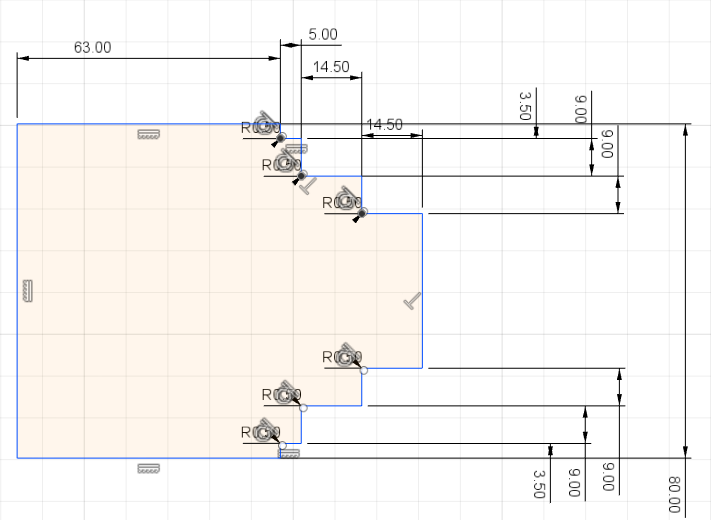
\includegraphics[width=110mm,keepaspectratio]{Figures/Placa1v6.png}
	\caption{Medidas de la placa electrónica.}
	\label{fig:medidaspcb}
\end{figure}

Una vez que fueron establecidas las medidas y el microcontrolador que debía ser usado (un msp430), se delimitó la placa en los dos sectores previamente mencionados. Esta división puede observarse en la figura \ref{fig:pcbbase}, ambas divisiones deberían encontrarse aisladas, por lo que se debía dejar cierto espacio entre el cobre.

\begin{figure}[h]
	\centering
	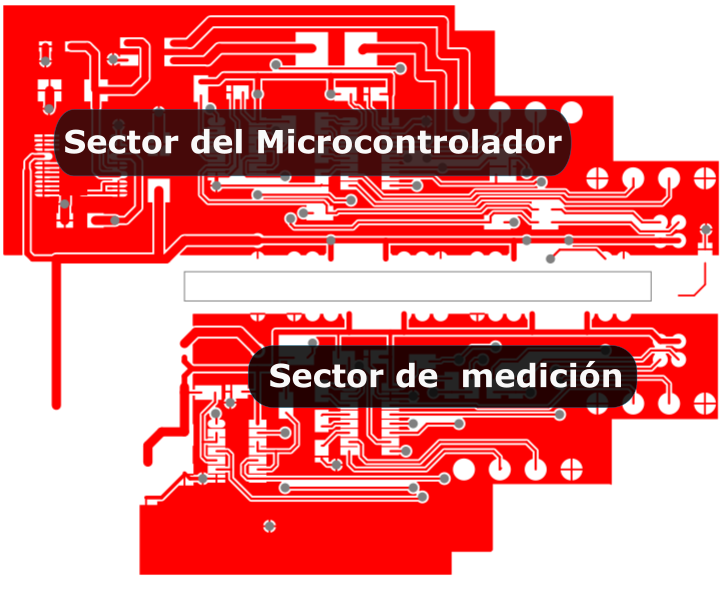
\includegraphics[width=80mm,keepaspectratio]{Figures/esquema22.png}
	\caption{Placa de ejemplo para la aislación.}
	\label{fig:pcbbase}
\end{figure}



La figura \ref{fig:pcbbase} es una vista de un diseño que proveyó la empresa como punto de partida para el desarrollo de los circuitos impresos.

Se estableció entonces que en el sector del microcontrolador se encontrarán los puertos de comunicación y en el sector de medición, los integrados y circuitos analógicos que adapten las entradas a medir.

\subsection{Componentes esenciales}

Basándose en los requerimientos se fue definiendo al dispositivo como  un conjunto de circuitos, estos son:

\begin{itemize}
\item Un circuito de alimentación.
\item Circuito de adaptación de microcontrolador.
\item Circuito de aislación, o de cambio de nivel.
\item Circuito de medición.
\item Circuito de comunicación por puerto.
\item Circuito de relé.
\item Circuito de salida analógica.
\end{itemize}

Todos estos circuitos se encuentran en el sector de microcontrolador que puede verse de la figura \ref{fig:pcbbase}, a excepción del circuito de  medición que se encuentra en el sector de medición  y el circuito de aislación que funciona de interface y se encuentra en ambos sectores.

\subsubsection{Circuito de alimentación}
Se comenzó a realizar el circuito teniendo por presupuesto que la alimentación se haría con una fuente alterna de 8 V a 30 V.

Para la alimentación se optó por una fuente switching  LM2574 que provee 5 V a un regulador lineal de 3,3 V necesarios para operar el microcontrolador. El circuito descrito puede observarse en la figura \ref{fig:circalim1}.

\begin{figure}[h]
	\centering
	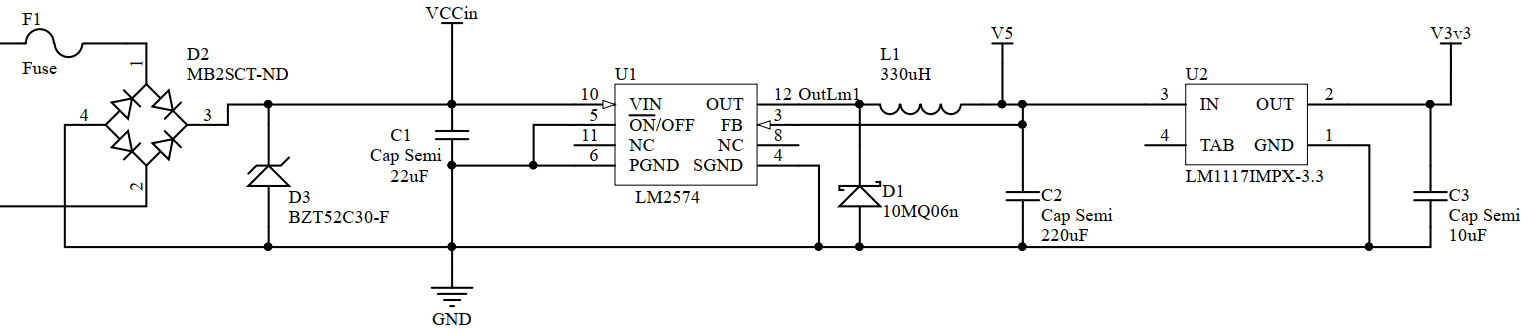
\includegraphics[width=120mm,keepaspectratio]{Figures/alimentacion1.png}
	\caption{Esquemático de la alimentación de la placa.}
	\label{fig:circalim1}
\end{figure}

\subsubsection{Circuito de aislación o de cambio de nivel}
Para proteger al microcontrolador de elevadas tensiones se utilizó un integrado de aislación, un conversor de continua a continua para alimentar el circuito de medición. También se añadió un aislador digital para comunicar el microcontrolador principal con un integrado de medición.

\begin{figure}[h]
	\centering
	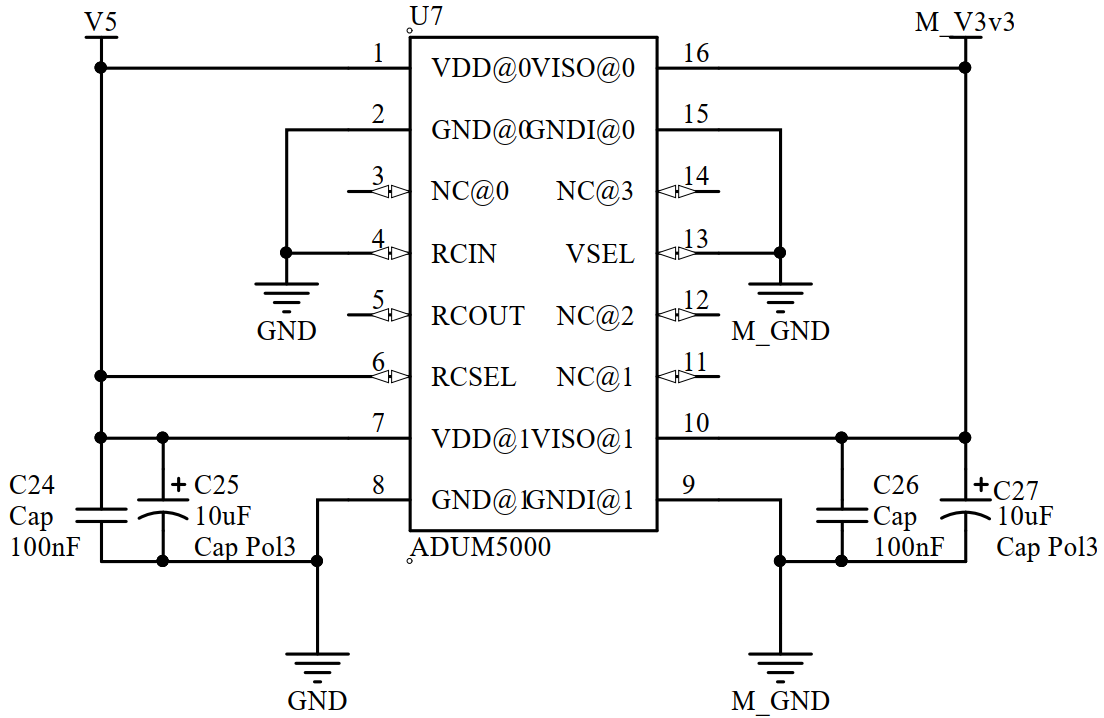
\includegraphics[width=100mm,keepaspectratio]{Figures/alimentacion2.png}
	\caption{Esquemático de la alimentación del sector aislado.}
	\label{fig:circaisl1}
\end{figure}

\begin{figure}[h]
	\centering
	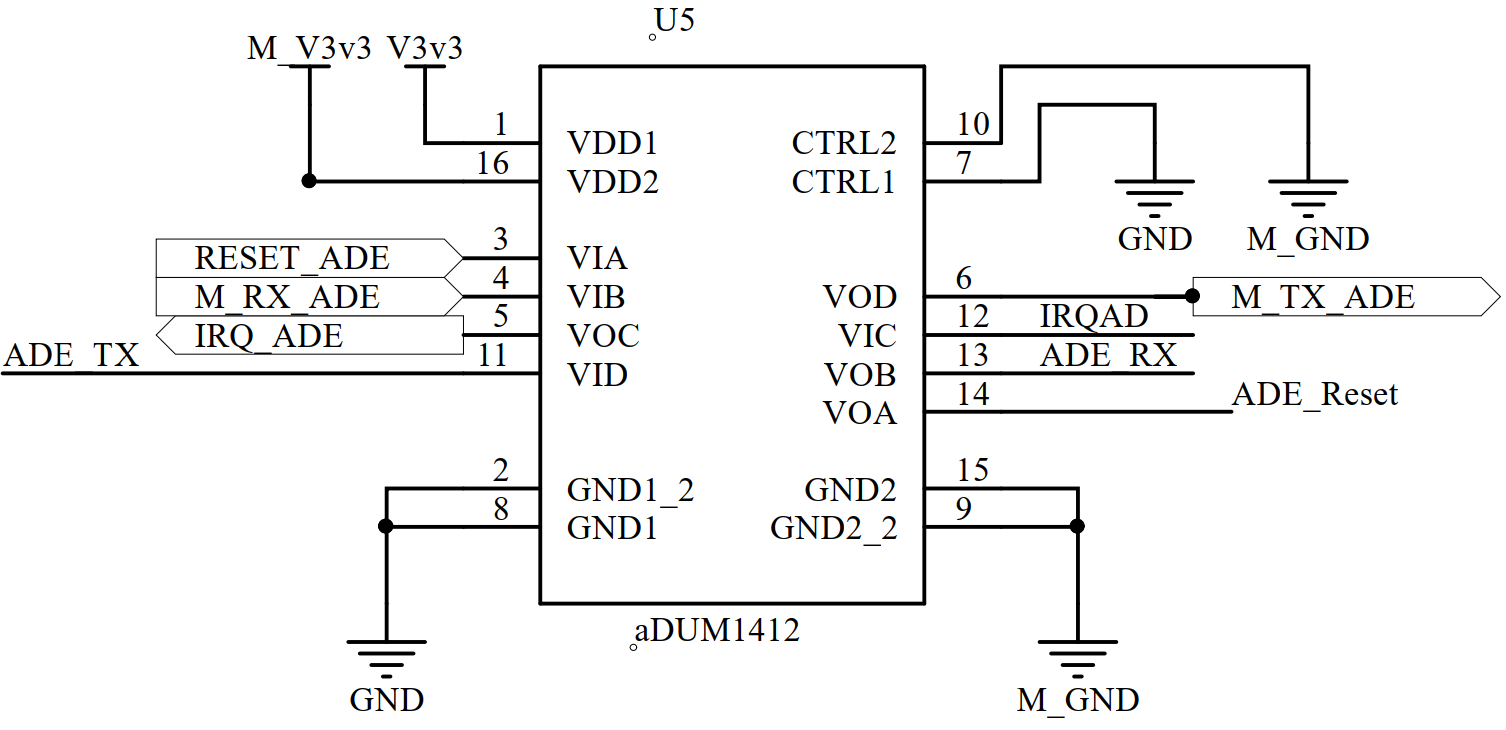
\includegraphics[width=100mm,keepaspectratio]{Figures/comaislado1.png}
	\caption{Esquemático de la comunicacion digital aislada.}
	\label{fig:circaisl2}
\end{figure}

 
\subsubsection{Circuito de adaptación de microcontrolador}

El circuito de adaptación esta integrado por resistores y capacitores necesarios para el correcto funcionamiento del microcontrolador, como tambien un cristal externo para usarlo como oscilador. Se usó un microcontrolador de la familia MSP430, este micro es de uso común en la empresa. 

En el circuito de adaptación se incluyó un semiconductor para tensión de referencia y un cristal de 32768 Hz. Para el armado del dispositivo se seleccionó el modelo msp430F2618, que posee un DAC interno de 12 bit que es de utilidad para la salida analógica utilizada en el lazo de corriente.

Para programar al microcontrolador se añadió una conexión JTAG para conectar un programador flash de la empresa Texas Instrument. Este puerto de salida puede verse en la figura \ref{fig:jitag}.

\begin{figure}[h]
	\centering
	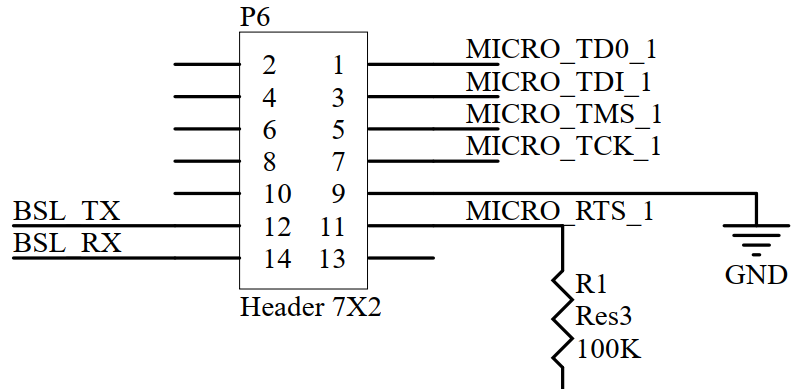
\includegraphics[width=120mm,keepaspectratio]{Figures/JTAG1.png}
	\caption{Header JTAG añadido al PCB.}
	\label{fig:jitag}
\end{figure}

\subsubsection{Circuito de comunicación por puerto}
Como se estableció en los requisitos, se implementaron integrados para la comunicación RS232, un max3222 y para la RS485, un integrado ISL83485. Estos integrados facilitan la adaptación de tensiones para lograr el estándar de comunicación deseado.

\begin{figure}[h]
	\centering
	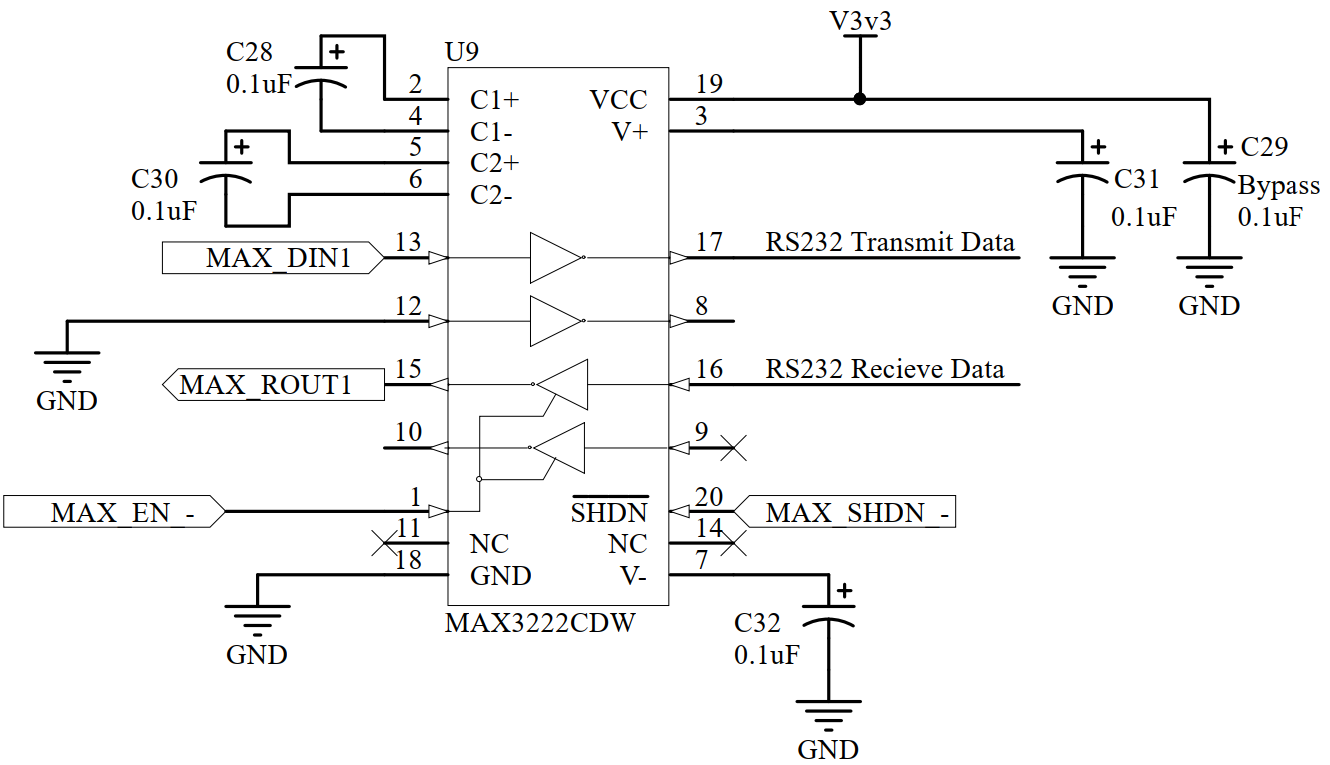
\includegraphics[width=120mm,keepaspectratio]{Figures/RSS232_1.png}
	\caption{Implementación del MAX3222 en el esquemático elaborado.}
	\label{fig:2321esquem}
\end{figure}

\begin{figure}[h]
	\centering
	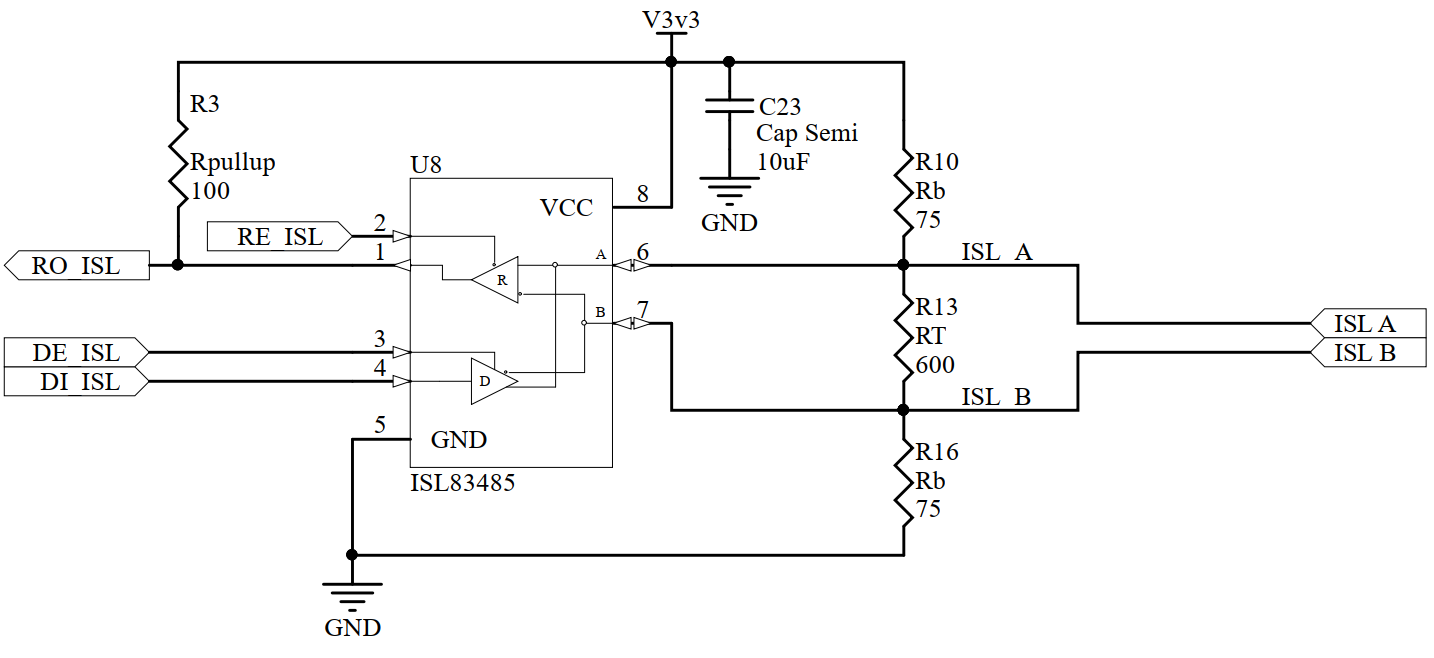
\includegraphics[width=120mm,keepaspectratio]{Figures/RSS485_1.png}
	\caption{Implementación del ISL83485 en el esquemático elaborado.}
	\label{fig:4851esquem}
\end{figure}


\subsubsection{Circuito de relé}
El circuito es integrado por los componentes mínimos para que el microcontrolador pueda manejar un relé que se acciona con tensiones del orden de los 5 volts. El circuito puede verse en la figura \ref{fig:rele1equem}.

\begin{figure}[h]
	\centering
	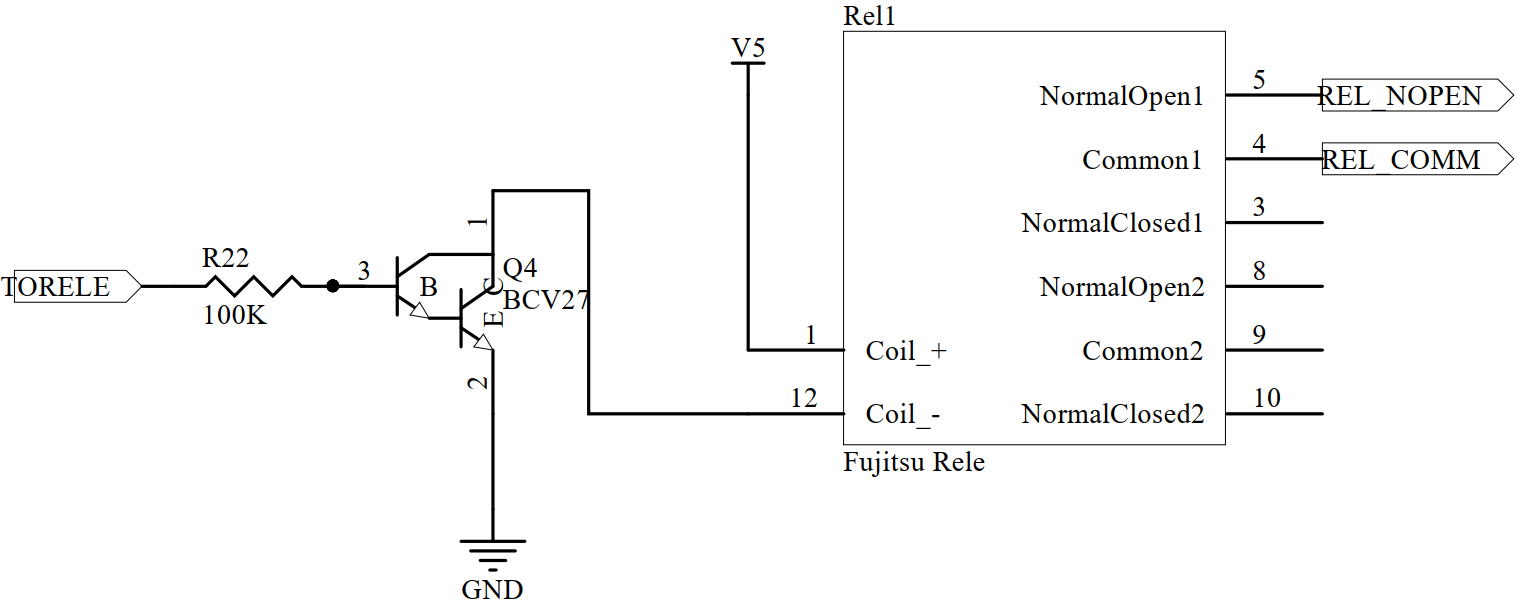
\includegraphics[width=120mm,keepaspectratio]{Figures/rele1.png}
	\caption{Transistor darlington para la acción del relé.}
	\label{fig:rele1equem}
\end{figure}

\subsubsection{Circuito de salida analógica}
Este circuito esta compuesto por un \textit{buffer} combinado con un integrado regulador de corriente para lograr una salida de lazo de corriente 4 - 20 mA.

\begin{figure}[h]
	\centering
	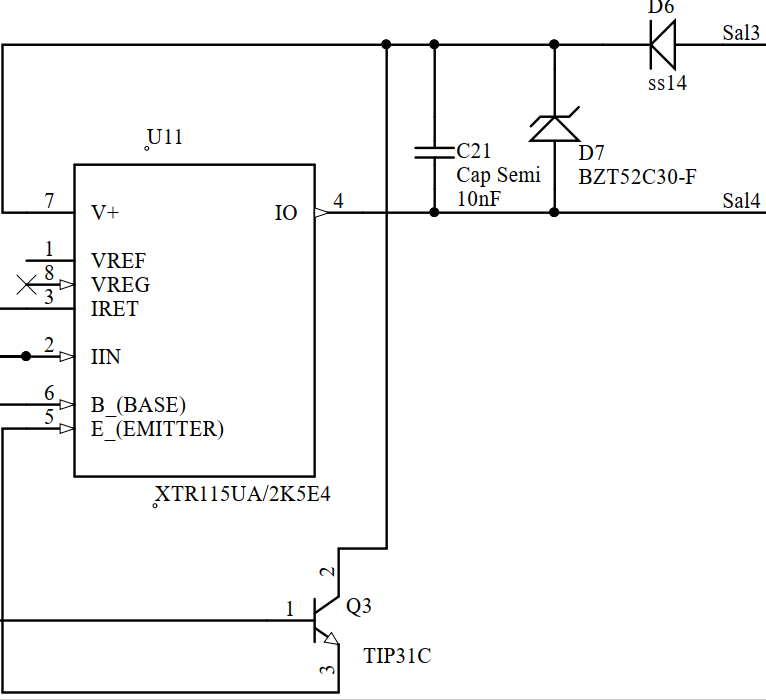
\includegraphics[width=120mm,keepaspectratio]{Figures/salida420.png}
	\caption{Circuito de salida 4 - 20 mA.}
	\label{fig:rele1equem}
\end{figure}


\subsubsection{Circuito de medición}

Para realizar la medición se optó por un integrado miltifuncional de medición de una sola fase. El  integrado permitió la rápida implementación de un medidor en el circuito del dispositivo. El integrado elegido es el ADE7953 del fabricante Texas Instrument. El integrado es un SOC (\textit{system on chip}) que adapta un AFE (\textit{analog front-end} ) para su fácil uso. El esquemático del ADE7953 puede verse en la  figura \ref{fig:ade79esquem}.

\begin{figure}[htb]
	\centering
	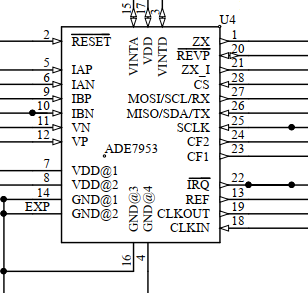
\includegraphics[width=100mm,keepaspectratio]{Figures/ade7953.png}
	\caption{Diagrama de bloque del ADE7953.}
	\label{fig:ade79esquem}
\end{figure}

El integrado de medición puede comunicarse con el microcontrolador por tres diferentes protocolos: I2C, SPI y UART, para esto deben realizarse las conexiones necesarias. Debido a la decisión de aislar el integrado y que las condiciones de espacio no permitían sobrepasarse con la cantidad de integrados para aislar, se realizaron las conexiones para la comunicación UART solamente.

\subsection{Esquema analógico de medición }
Como el principal objetivo del dispositivo es medir, se explica de manera muy breve, los arreglos analógicos que se implementaron.

Suponiendo que las tensiones a medir fuesen del orden de los 600 V y teniendo en cuenta que la máxima tension que soporta un pin del integrado es de 2 V, se añadió una serie de resistores para lograr 1 mega $\Omega$  de resistencia en la entrada de medición, de modo de atenuar la tension. Una vez atenuada la tensión se agrega un divisor resistivo del cual el integrado mide.

\begin{figure}[htb]
	\centering
	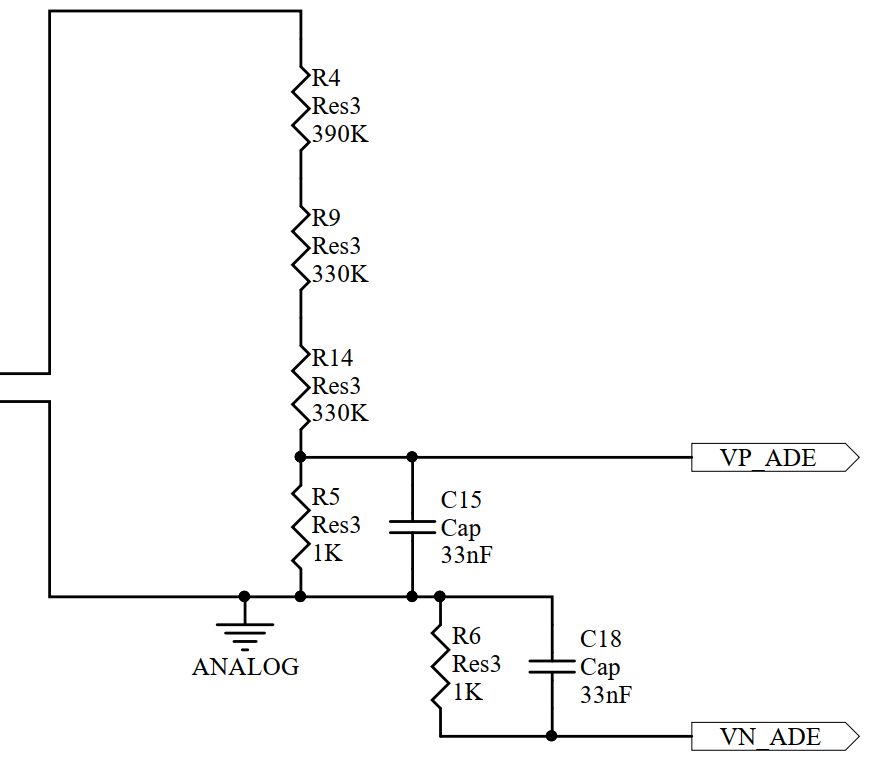
\includegraphics[width=80mm,keepaspectratio]{Figures/medicionvoltaje.png}
	\caption{Esquemático de la entrada de tension.}
	\label{fig:medvolt}
\end{figure}

Para la medición de corriente es común ver en los módulos comerciales el uso de una bobina de Rogowski, sin embargo para el modulo diseñado se optó por usar un \textit{shunt} para que el dispositivo no dependa de otro objeto discreto para su instalación. El \textit{shunt} elegido soporta grandes corrientes y se tomaron precauciones en las pistas del PCB para que pueda operar con normalidad.

\begin{figure}[htb]
	\centering
	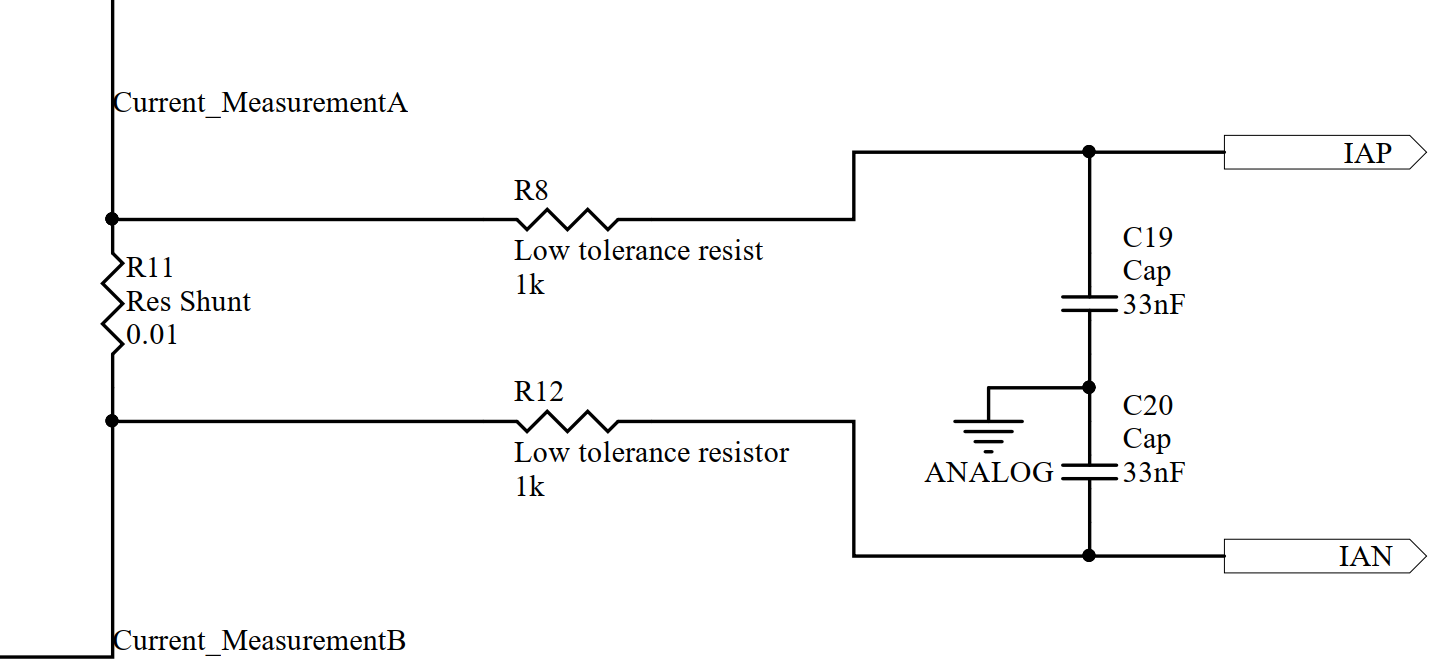
\includegraphics[width=120mm,keepaspectratio]{Figures/medicioncorriente.png}
	\caption{Esquemático de la entrada de corriente.}
	\label{fig:medcurrent}
\end{figure}

\subsection{Fabricación}

Una vez completada la totalidad de las conexiones lógicas en el esquemático, se debía decidir sobre el posicionamiento de los componentes, el tamaño de las perforaciones y la distribución de cada circuito. Se estableció desde la empresa privada que todos los componentes pasivos en lo posible sean de montaje superficial, por lo que la mayoría de resistores y capacitores serian de encapsulado 0805. Un 0805 puede verse en la figura \ref{fig:smd0805}.

\begin{figure}[!h]
	\centering
	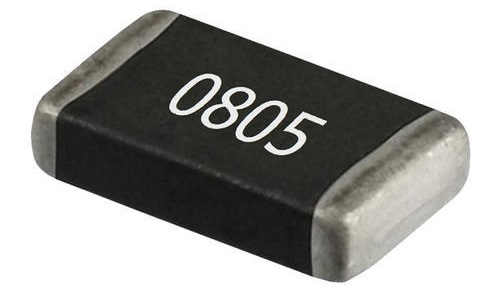
\includegraphics[width=50mm,keepaspectratio]{Figures/smd0805.jpg}
	\caption{Componente de soldadura superficial.}
	\label{fig:smd0805}
\end{figure}

Se dejó espacio para una entrada de conector RJ45 para un futuro puerto LAN ethernet y se delimitó una zona de exclusión para dividir al PCB en una zona de medición y una zona de microcontrolador.

Debido a que el PCB iba a ser encapsulado por una carcasa de plástico con posibilidad de conexión de 16 salidas, se decidió previamente como debería ser el esquema de conexiones. Se dejo un conector de 4 salidas para las mediciones ya que este se encontraría en un nivel aislado.

\begin{figure}[h]
	\centering
	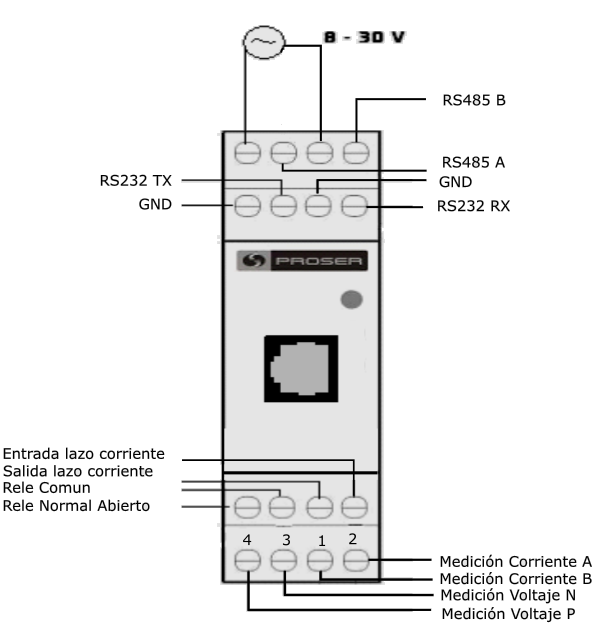
\includegraphics[width=120mm,keepaspectratio]{Figures/conectores2.png}
	\caption{Salidas del dispositivo.}
	\label{fig:salidas01}
\end{figure}

Se decidió fabricar las placas electrónicas en Argentina. La empresa fabricante tiene publicada una tabla donde divulga con qué tipos de tecnología de fabricación trabaja. Se estableció como estándar a usar el de 8 milis y se trabajó con ese limite en el CAD de diseño.

\begin{figure}[htb]
	\centering
	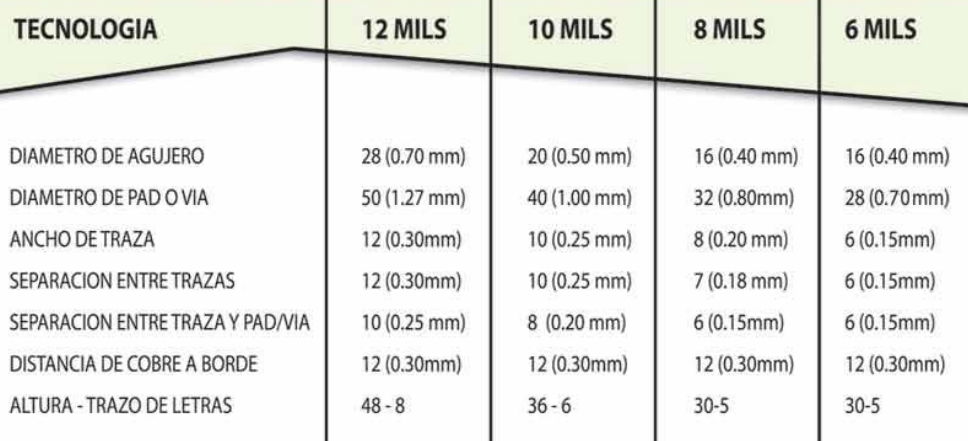
\includegraphics[width=110mm,keepaspectratio]{Figures/estandaresmayer.png}
	\caption{Estandares fijados por la empresa argentina Ernesto Mayer SA.}
	\label{fig:mayerstandar}
\end{figure}

El resultado del diseño puede verse en la figura \ref{fig:PCBfrontt}, que es la cara superior de la placa donde se encuentran la mayoría de los componentes. 

\begin{figure}[h]
	\centering
	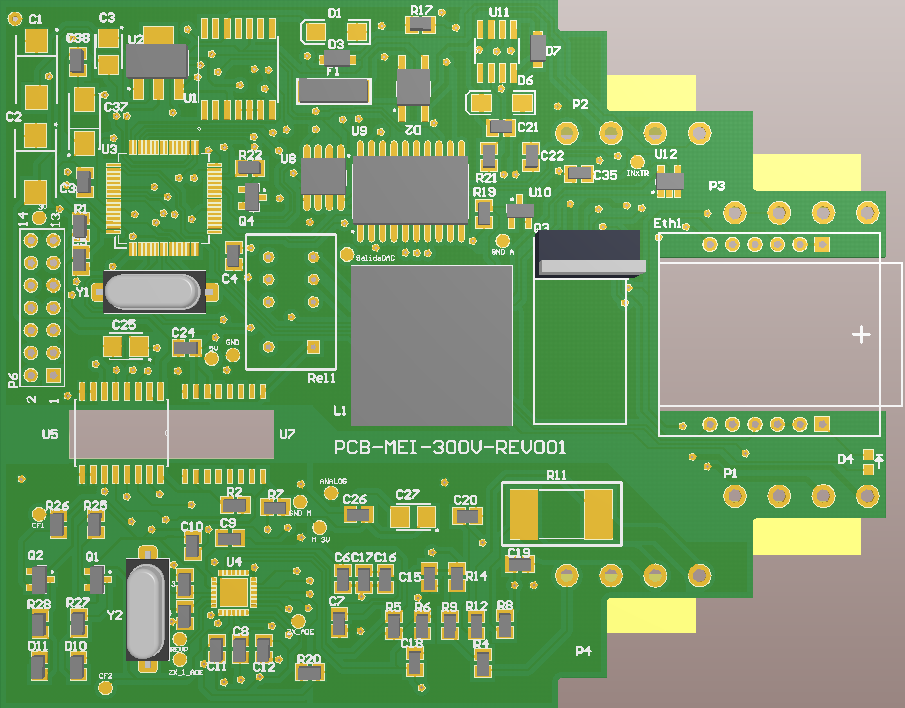
\includegraphics[width=110mm,keepaspectratio]{Figures/PCBfront.png}
	\caption{Imagen 3D de la parte frontal del PCB.}
	\label{fig:PCBfrontt}
\end{figure}

La cara inferior puede verse en la figura \ref{fig:PCBbackk}. Como esta cara se soldaría por refusión de una ola de estaño que viene de izquierda a derecha, tal como se ve a la imagen, se minimizó la cantidad de integrados en ella y se acomodaron los \textit{footprints} para que no queden puntos ciegos sin soldar.

\begin{figure}[htb]
	\centering
	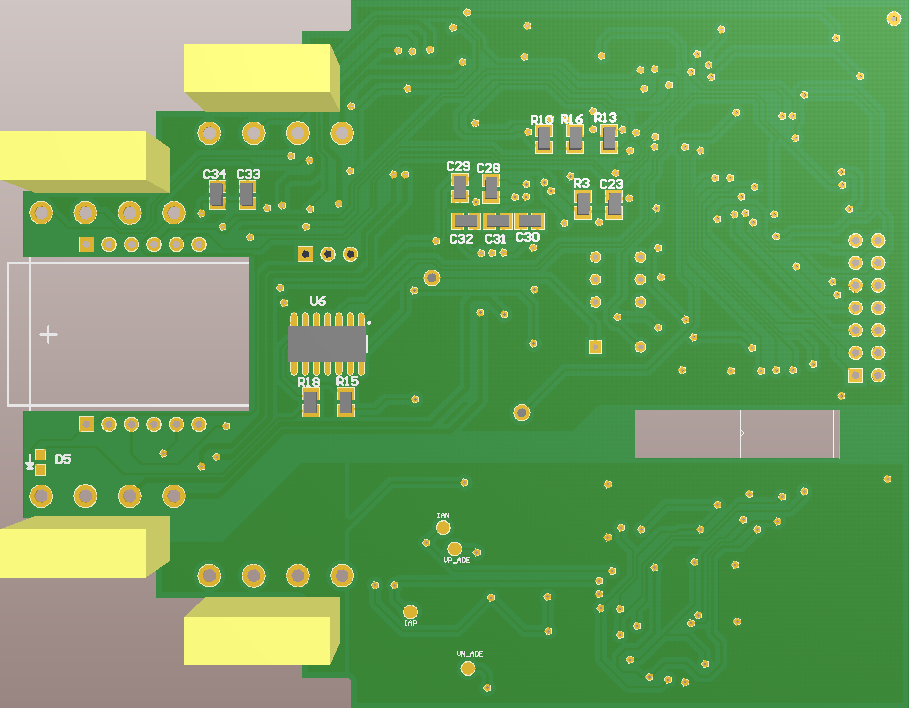
\includegraphics[width=110mm,keepaspectratio]{Figures/PCBback.png}
	\caption{Imagen 3D de la parte trasera del PCB.}
	\label{fig:PCBbackk}
\end{figure}


\section{Desarrollo de \textit{software}}
Se desarrollo un software para e uso del dispositivo armado, es decir se desarrollo un programa en c para descargarlo al microcontrolador y que este realice todas las tareas necesarias.

\subsection{Software previos de base}
Se desarrollo durante la cursada de la especialización un programa en lenguaje c para implementarlo en un microntrolador LPC4337 para hacer uso de un circuito integrado wiznet w5500, que es un controllador ethernet que maneja protocolo TCP/IP, comunmente utilizado para realizar una conecxion a internet de manera sencilla. Se penso en el desarrollo de este programa para implementarlo al futuro puerto ethernet del dispositivo.

También se habían desarrollado como parte de las materias de la especialización programas simples de bucle infinito con interrupción para la introducción de sistemas operativos, uno de estos programas fue usado como base para la elaboración del programa final.


\subsection{Microcontrolador Principal}
El microcontrolador elegido para el dispositivo fue un MSP430F2618 fabricado por la empresa Texas Instrument, este microcontrolador es de ultra baja potencia con una CPU de instrucciones RISC de 16 bits. Posee periféricos analógicos y digitales orientado a aplicaciones de medición. Este microcontrolador puede pasar de varios modos de baja potencia a modo activo en menos de 1 microsegundo.

\begin{figure}[!h]
	\centering
	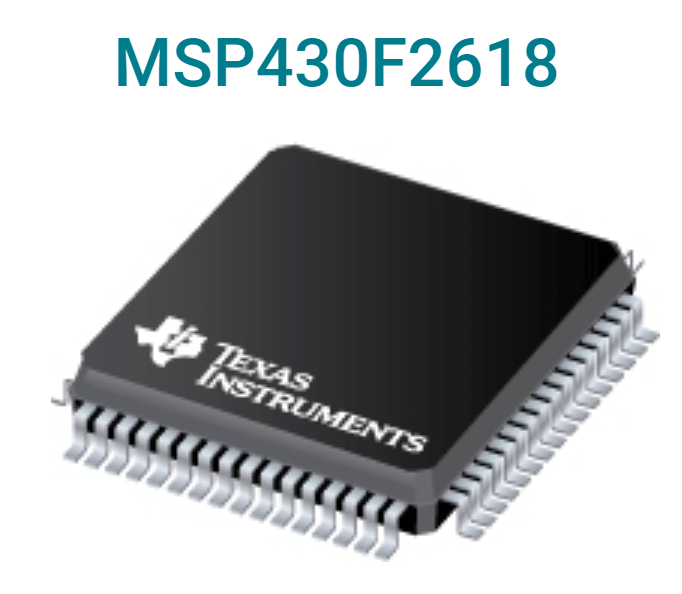
\includegraphics[width=40mm,keepaspectratio]{Figures/msp430F2618.png}
	\caption{Ilustración del micro controlador como se lo presenta en la pagina web del fabricante.}
	\label{fig:msp430imagen}
\end{figure}

Para realizar el programa en lenguaje c y descargarlo en el microcontrolador la empresa SERVAIND S.A. proveyó un entorno de desarrollo privado y una placa electrónica con el microcontrolador funcionando, de modo de probarla. Una ventana del entorno de desarrollo puede verse en la figura \ref{fig:IARwindow}.

\begin{figure}[h]
	\centering
	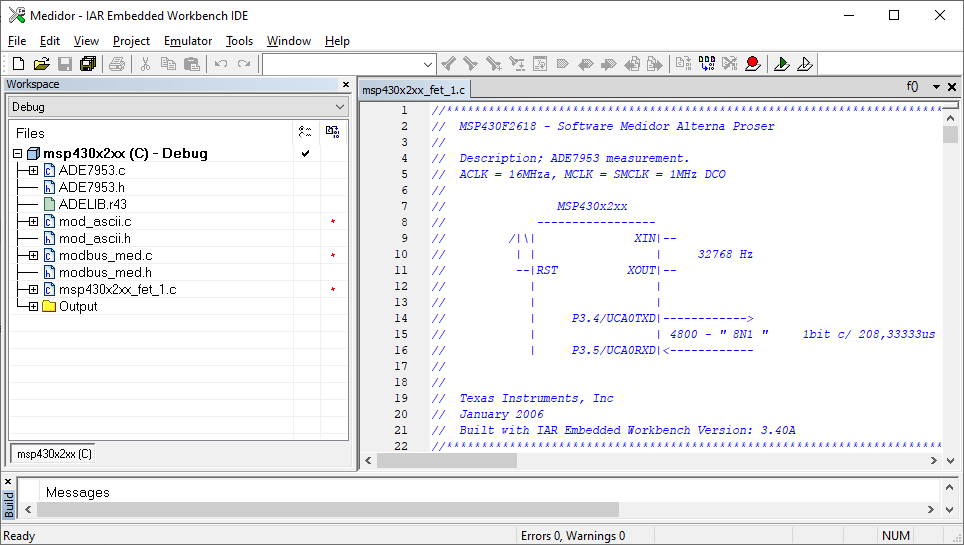
\includegraphics[width=110mm,keepaspectratio]{Figures/Embeddedworkbench.png}
	\caption{Imagen del entorno de desarrollo.}
	\label{fig:IARwindow}
\end{figure}



\subsection{Especificaciones del software desarrollado}

Ante la necesidad de realizar un software robusto y de uso instrumental se deseaba implementar un FreeRTOS pero  debido a limitaciones de memoria del microcontrolador resultaba inviable implementarlo, por lo que se decidió realizar un programa \textit{bare metal}.

El software realizado consiste en un bucle infinito controlado por tiempo(1 milisegundo) usando uno de los dos timers internos del microcontrolador. La principal tarea del programa es comunicarse constantemente con el integrado de medición \textbf{ADE7953} y almacenar los datos de sus registros en la memoria local. Dentro del periodo de un milisegundo que dura el barrido del bucle se realizan otras tareas como comunicar datos a otros puertos, accionar el relé o cambiar los leds.

\subsubsection{Comunicacion con el ADE7953}

La comunicación con el ADE7953 se realiza por UART por medio de un protocolo establecido por el fabricante del chip. Como la comunicación UART del chip esta fijada en 4800 bps cada frame que se le envía tiene un tiempo de 2.08 ms, el tiempo entre cada frame es de 0.2 ms a 4ms (t1) como máximo y el tiempo de espera entre cada comunicación exitosa es de 6ms (t2).

El ADE7953 tiene registros internos de 8, 16 y 24 bits donde almacena información de medición y de configuración para su funcionamiento, estos registros son tanto de escritura como de lectura. La dirección  de registros de 8 bits puede verse en la tabla \ref{8biadcregis}.

Las operaciones de lectura con el ADE7953 puede verse en la figura \ref{fig:ADEread}, para leer un registro debe primeramente enviarse un byte de valor 0x35 y luego los bytes de la dirección del registro a leer, para luego recibir la cantidad de bytes según el tamaño del registro solicitado.

\begin{figure}[htb]
	\centering
	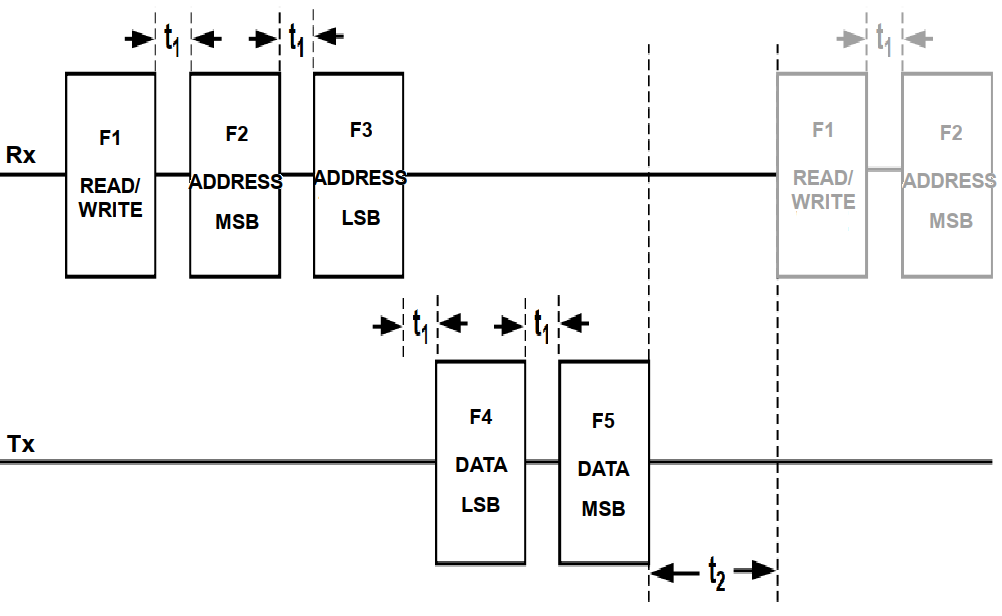
\includegraphics[width=110mm,keepaspectratio]{Figures/ade7uartread.png}
	\caption{Lectura por UART del ADE7953.}
	\label{fig:ADEread}
\end{figure}

Para la operación de escritura del ADE7953 debía enviarse un byte con el valor 0xCA ,luego los bytes de la dirección a escribir y por ultimo los datos en la misma cantidad de \textit{frames} que espacio del registro, como puede observarse en la figura \ref{fig:ADEwrite}.

\begin{figure}[htb]
	\centering
	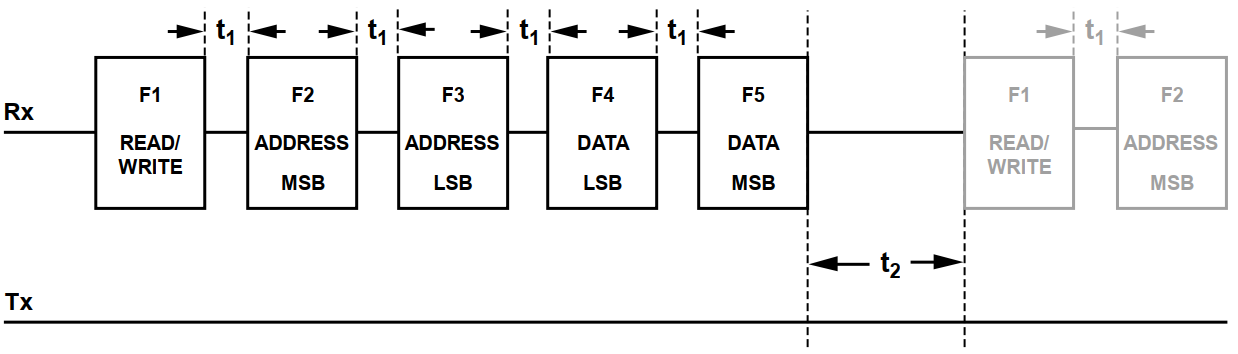
\includegraphics[width=110mm,keepaspectratio]{Figures/ade7uartwrite.png}
	\caption{Escritura por UART del ADE7953.}
	\label{fig:ADEwrite}
\end{figure}

Se configuro al programa de tal modo que lea los registros necesarios para monitorear la potencia eléctrica de la maquina donde se lo instale, los registros que el programa lee y almacena son:

\begin{itemize}
\item AVA\_ 24 Potencia aparente instantánea. 
\item AWATT\_ 24 Potencia activa instantánea.
\item AVAR\_ 24 Potencia reactiva instantánea. 
\item IA\_ 24 Corriente instantánea.
\item V\_ 24 Voltaje instantáneo.
\item IRMSA\_ 24 Corriente RMS.
\item VRMS\_ 24 Voltaje RMS.
\item AENERGYA\_ 24 Energia activa.
\item RENERGYA\_ 24 Energia reactiva.
\item APENERGYA\_ 24  " Energía Aparente".
\item VPEAK\_ 24 Pico de voltaje.
\item PFA\_ 16 Factor de potencia.
\item Period\_ 16 Registro de período.
\end{itemize}


El programa tarda aproximadamente un total de 241 ms en leer la totalidad de estos registros usando el protocolo elegido, por lo que queda un amplio margen para realizar otras operaciones.


\begin{table}[h]
\centering
\caption[Registros 8 bit ADE79853]{Registros de 8 bit del ADE7953 como se los muestran en el \textit{datasheet} del fabricante.}
\begin{tabular}{@{}llllll@{}}
\hline
Address & Register Name  & R/W & Default & Type     & Register Description                                                                                                                                 \\ \hline
0x000   & SAGCYC         & R/W & 0x00    & Unsigned & Sag line cycles                                                                                                                                      \\
0x001   & DISNOLOAD      & R/W & 0x00    & Unsigned & No-load detection disable                                                                                                                            \\
0x004   & LCYCMODE       & R/W & 0x40    & Unsigned & \begin{tabular}[c]{@{}l@{}}Line cycle accumulation mode \\ configuration\end{tabular}                                                                \\
0x007   & PGA\_V         & R/W & 0x00    & Unsigned & \begin{tabular}[c]{@{}l@{}}Voltage channel \\ gain configuration (Bits{[}2:0{]})\end{tabular}                                                        \\
0x008   & PGA\_IA        & R/W & 0x00    & Unsigned & \begin{tabular}[c]{@{}l@{}}Current Channel A\\  gain configuration (Bits{[}2:0{]})\end{tabular}                                                      \\
0x009   & PGA\_IB        & R/W & 0x00    & Unsigned & \begin{tabular}[c]{@{}l@{}}Current Channel B gain \\ configuration (Bits{[}2:0{]})\end{tabular}                                                      \\
0x040   & WRITE\_PROTECT & R/W & 0x00    & Unsigned & \begin{tabular}[c]{@{}l@{}}Write protection bits\\  (Bits{[}2:0{]})\end{tabular}                                                                     \\
0x0FD   & LAST\_OP       & R   & 0x00    & Unsigned & \begin{tabular}[c]{@{}l@{}}Contains the type \\ (read or write) \\ of the last successful \\ communication\\ (0x35 =read; 0xCA = write)\end{tabular} \\
0x0FF   & LAST\_RWDATA   & R   & 0x00    & Unsigned & \begin{tabular}[c]{@{}l@{}}Contains the data from \\ the last successful 8-bit\\  register communication\end{tabular}                                \\
0x702   & Version        & R   & N/A     & Unsigned & \begin{tabular}[c]{@{}l@{}}Contains the silicon\\  version number\end{tabular}                                                                       \\
0x800   & EX\_REF        & R/W & 0x00    & Unsigned & \begin{tabular}[c]{@{}l@{}}Reference input \\ configuration: set\\  to 0 for internal; \\ set to 1 for external\end{tabular}                         \\ \hline
\end{tabular}
\label{8biadcregis}
\end{table}




\subsection{Funcionalidades del software}
El software maneja un menú por el cual una terminal puede comunicarse con el programa por medio de un puerto serie para realizar determinadas configuraciones.

Al iniciar el programa, dentro de los primeros 10 segundos se puede enviar unos caracteres en código ANSII (las letras cfg) y el programa inicia un menú, enviando caracteres con las opciones. Este menú puede verse en la figura  \ref{fig:menumanual}.

El menú puede mostrar las variables que se están midiendo configurar el puerto serie, modificar a que variable depende la salda del bucle analógico y activar una alarma que acciona al relé dependiendo de una variable seleccionada.

\begin{figure}[!htb]
	\centering
	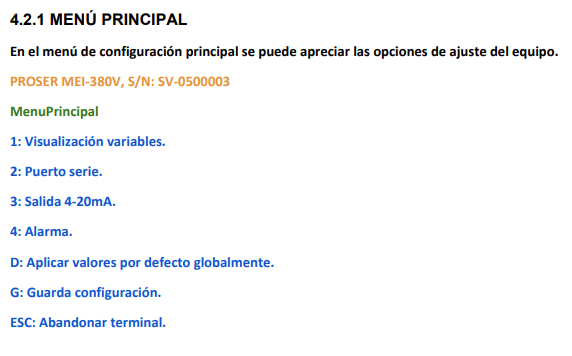
\includegraphics[width=110mm,keepaspectratio]{Figures/menumanual.png}
	\caption{Menú serie en el manual.}
	\label{fig:menumanual}
\end{figure}

\begin{figure}[!htb]
	\centering
	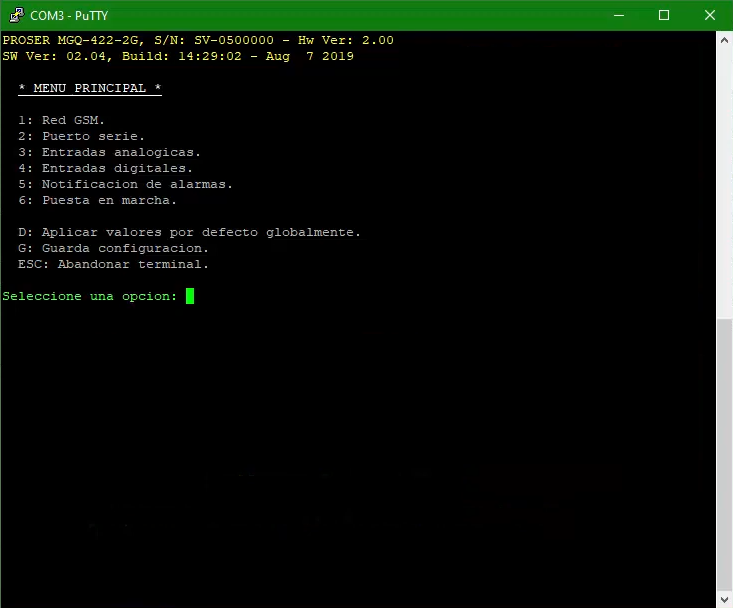
\includegraphics[width=110mm,keepaspectratio]{Figures/menudispositivo07.png}
	\caption{Menú serie ejemplo.}
	\label{fig:serialmenu}
\end{figure}

El software almacena en la memoria del programa valores de medición para poder comunicarlos ya sea por los puertos serie o el enlace de corriente.

El software que controla la placa maneja protocolo modbus para comunicar registros internos en 2 diferentes puertos de interfaces rs232 y 485 según sean seleccionados. Para implementarlo se siguió como referencia el "Modicon Modbus Protocol Reference Guide PI–MBUS–300" y un \textit{driver} libre, el freemodbus.

El modo de acceder a los datos por modbus es solicitando registros que el software maneja, la direccion de los registros puede verse en la tabla\ref{registrosmodbs}.

\begin{table}[h]
\caption[Registros modbus en software]{Registros generados para la comunicación modbus.}
\begin{tabular}{@{}lllll@{}}
\toprule
\begin{tabular}[c]{@{}l@{}}Dirección \\ del \\ Registro\end{tabular} & \begin{tabular}[c]{@{}l@{}}Número \\ del\\ parámetro\end{tabular} & Descripción                    & Unidades & Tipo de dato \\ \midrule
7001                                                                 & 1                                                                 & Voltaje Instantaneo            & Volts    & Float 32     \\
7003                                                                 & 2                                                                 & Voltaje rms                    & Volts    & Float 32     \\
7005                                                                 & 3                                                                 & Corriente instantánea          & Ampere   & Float 32     \\
7007                                                                 & 4                                                                 & Corriente rms                  & Ampere   & Float 32     \\
7009                                                                 & 5                                                                 & Potencia activa                & Watt     & Float 32     \\
7011                                                                 & 6                                                                 & Potencia reactiva              & VA       & Float 32     \\
7013                                                                 & 7                                                                 & Factor de potencia             & -        & Float 32     \\
7015                                                                 & 8                                                                 & Frecuencia                     & Hz       & Float 32     \\
7017                                                                 & 9                                                                 & Energía reactiva medida        & Joules   & Float 32     \\
7019                                                                 & 10                                                                & Energía activa Total acumulada & kWh      & Float 32    
\end{tabular}
\label{registrosmodbs}
\end{table}

EL sofware  maneja una salida para una conexión de lazo de corriente de 4 a 20 mili amperes que es un estándar en la industria para el control de procesos,  el programa puede hacer que esta salida sea proporcional a una variable de medición que puede seleccionarse en el menú serie de configuración.
